\chapter{Results and Analysis\label{ch:results}}

\section{Sensor Testing}
	In order to correctly apply Gaussian noise to the sensor measurements during the prediction step, we need to model the performance of the sensors. Additionally, we must determine the accuracy of the augmented reality tag detection for use in the weighting function of the correction step.

	\subsection{Gyroscope}
		The gyroscope was tested by placing the AR.Drone on a flat surface and recording the measured yaw angle. These readings were then centered about the mean and are shown in Figure~\ref{fig:gyr}.

		\begin{figure}[ht]
		        \centering
				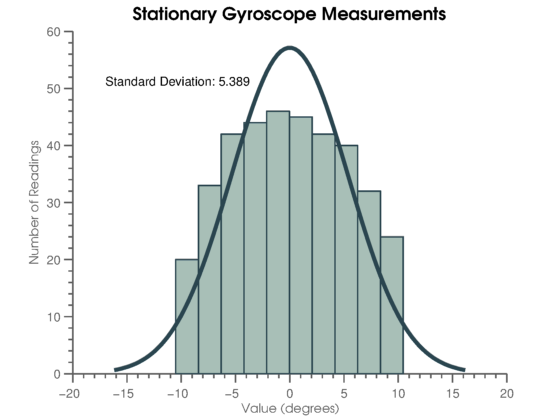
\includegraphics[width=300px]{../images/gyr_test.png}
				\caption{Stationary gyroscope test.}\label{fig:gyr}
		\end{figure}

	\subsection{Ultrasound Altimeter}

		The best way to test the ultrasound altimeter would be to attach the AR.Drone to a stationary rig and take measurements at several different heights within the operating range. Unfortunately, the AR.Drone SDK does not provide direct access to the ultrasound sensor and returns a value of zero if the quadcopter is not currently flying. Therefore, the ultrasound altimeter was tested by hovering the quadcopter at a constant height in a controlled, indoor environment. While some of the noise in the sensor measurement is due to the quadcopter actually changing altitude, these measurements (Figures~\ref{fig:ultra1} and~\ref{fig:ultra2}) still give us a general idea of the accuracy of the sensor.

		\begin{figure}[ht]
		        \centering
		        \begin{subfigure}[b]{0.45\textwidth}
		                \centering
		                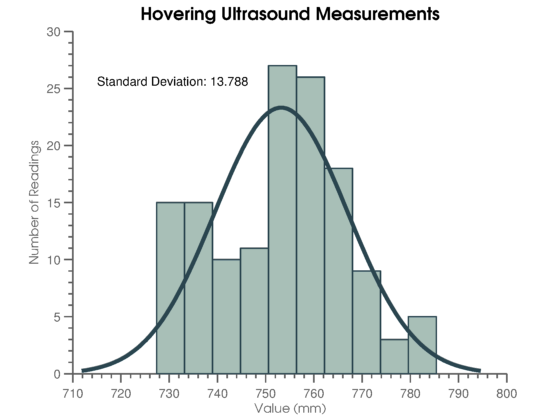
\includegraphics[width=\textwidth]{../images/ultra_test1.png}
		                \caption{Hovering at approximately 700mm}\label{fig:ultra1}
		        \end{subfigure}%
		        ~
		        \begin{subfigure}[b]{0.45\textwidth}
		                \centering
		                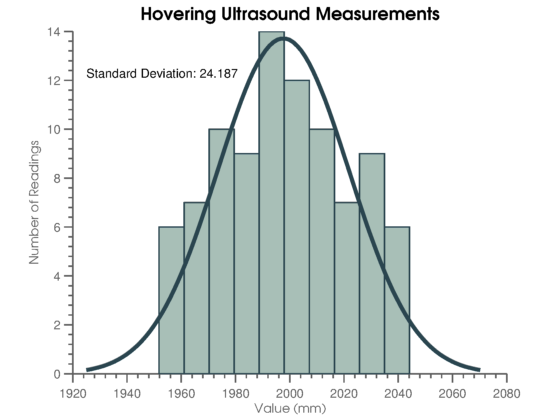
\includegraphics[width=\textwidth]{../images/ultra_test2.png}
		                \caption{Hovering at approximately 2000mm}\label{fig:ultra2}
		        \end{subfigure}
		        \caption{Hovering ultrasound test.}
		\end{figure}

	\subsection{Augmented Reality Tag Detection}

		\subsubsection{Detection Range}

			The quadcopter was mounted horizontally to test different aspects of the AR tag detection (Figure~\ref{fig:rig}). In determining the size of tag to use, there were two main considerations. The smaller the tags, the earlier they could be detected in the takeoff sequence, which is when visual localization performs poorly and it is especially important to use a tag for correction. On the other hand, if the tags were too small, then the altitude at which it could be detected would be too limited. We chose a tag size of 135cm, which we found to have a detection range of approximately 30cm to 4m (Figure~\ref{fig:extremes}). In order to increase the operational range of the AR tag correction, we could potentially use a combination of tags of different sizes.

			\begin{figure}[ht]
			        \centering
					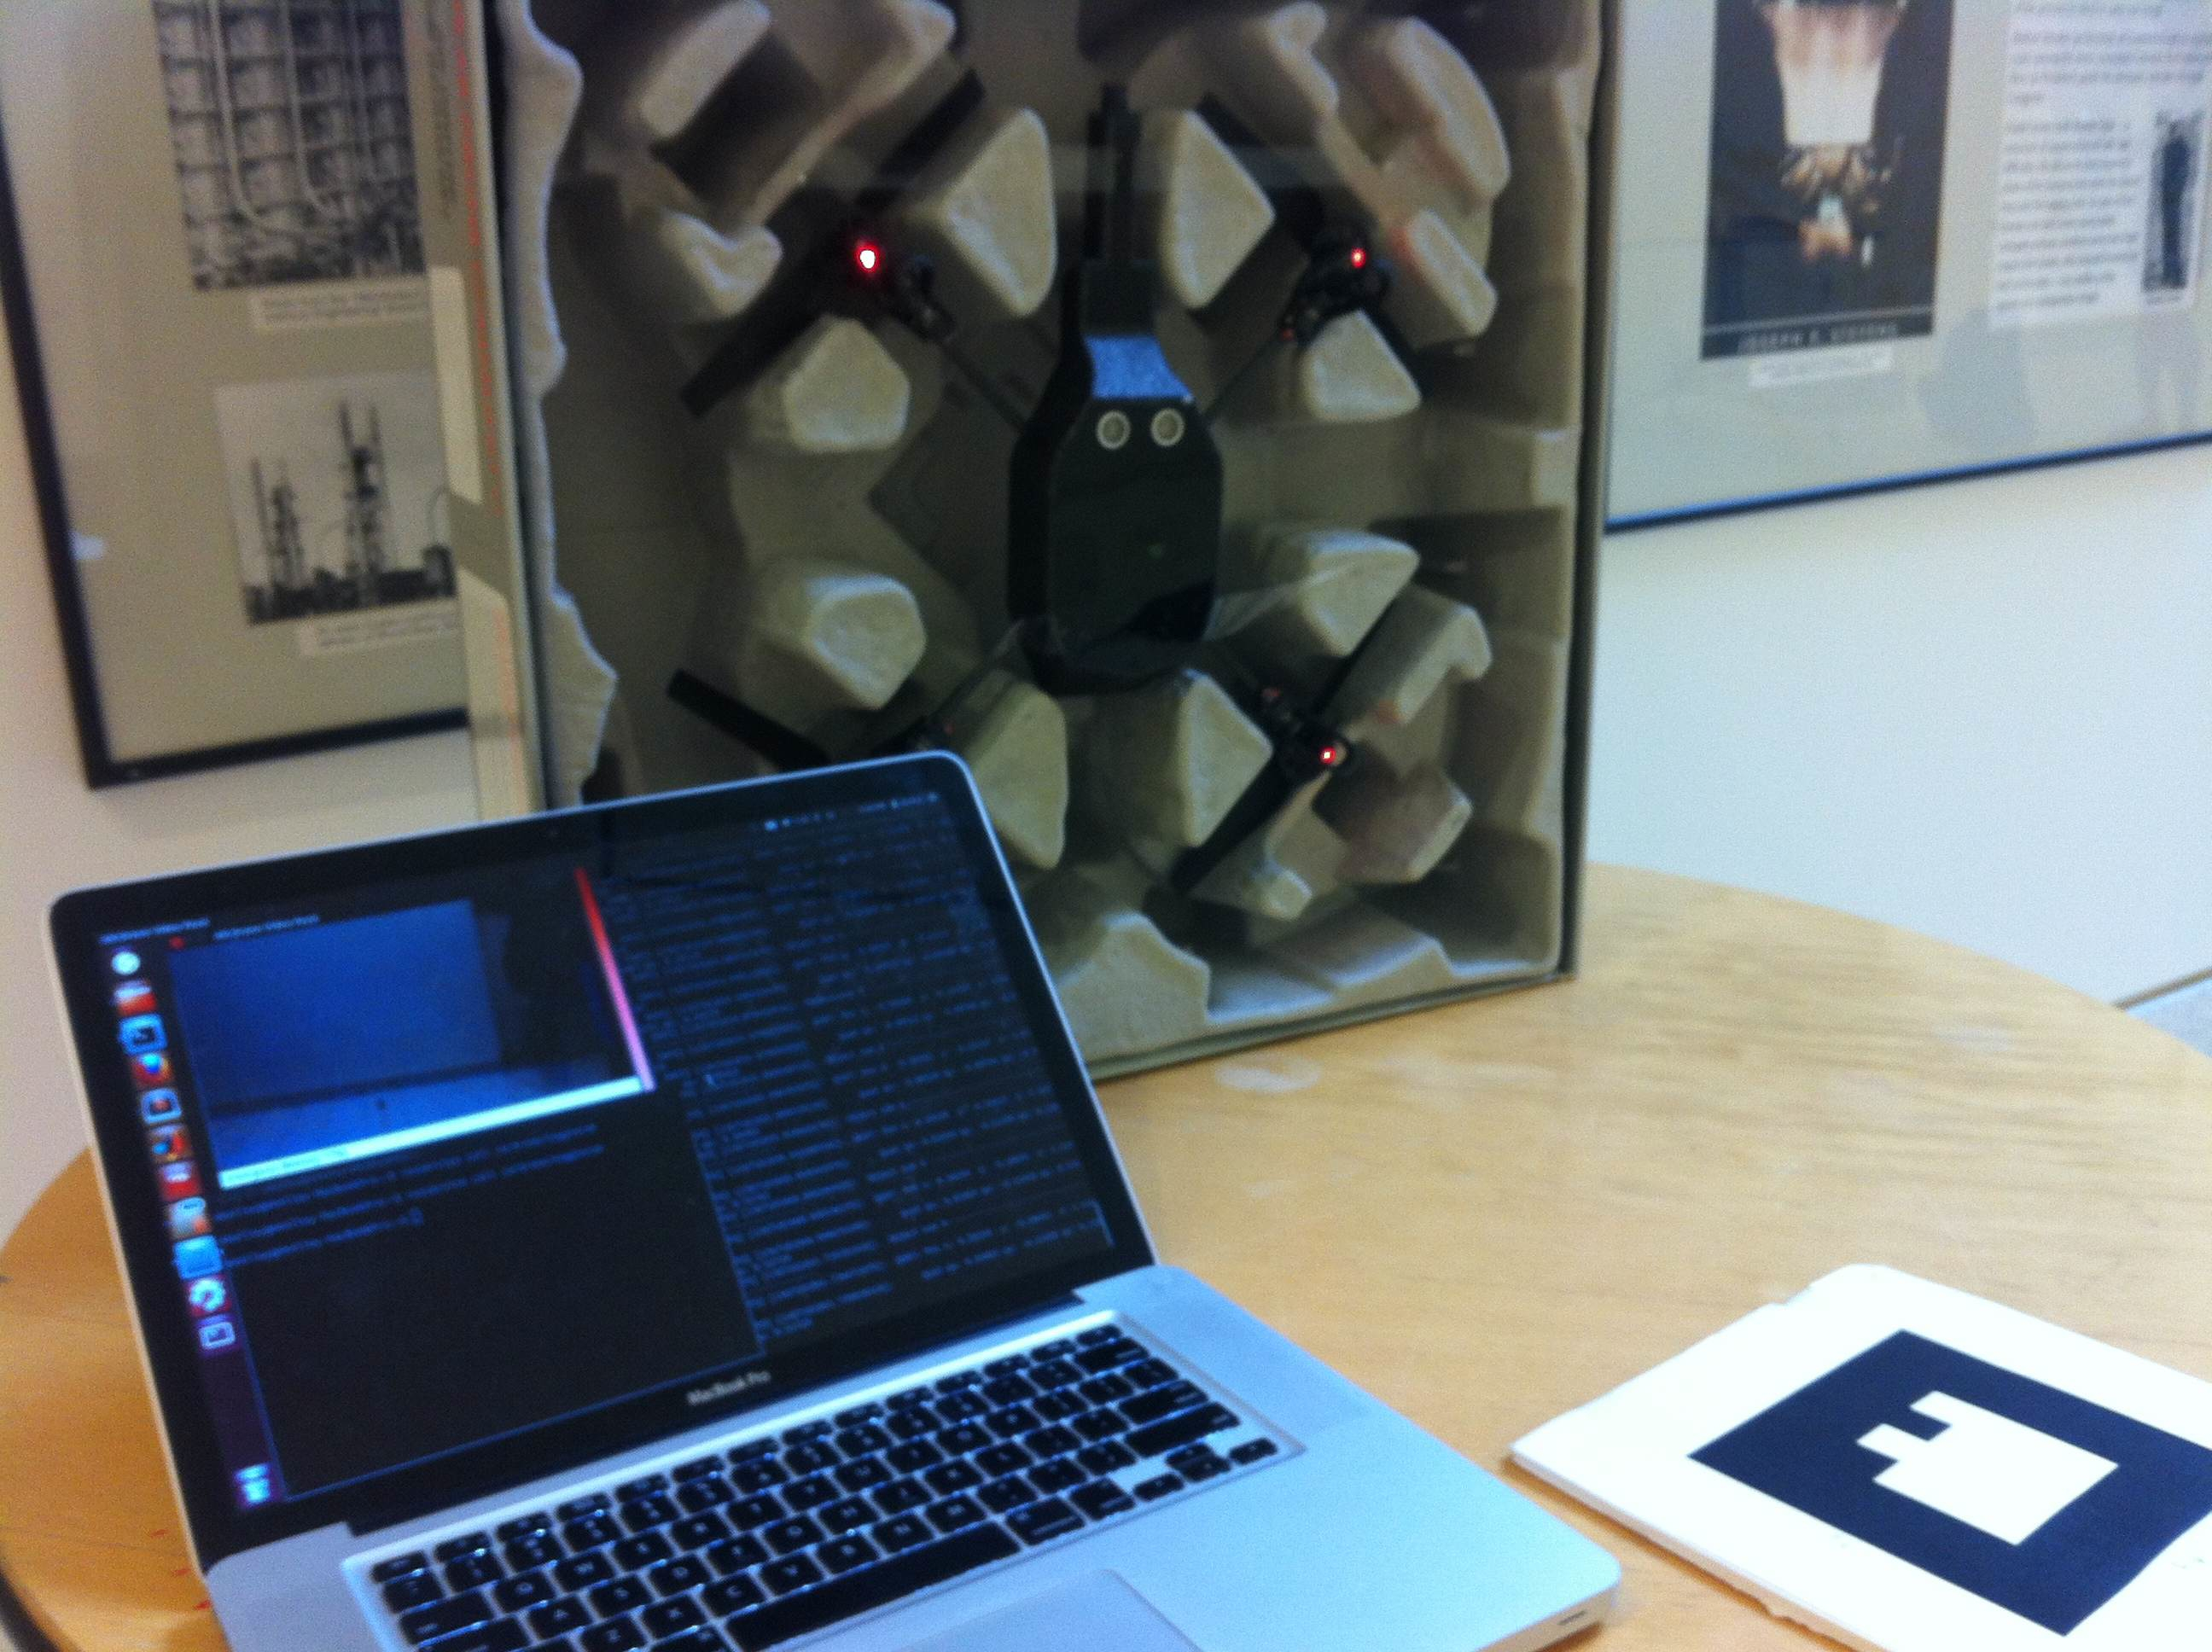
\includegraphics[width=200px]{../images/rig.jpg}
					\caption{AR tag testing setup.}\label{fig:rig}
			\end{figure}

			\begin{figure}[ht]
			        \centering
			        \begin{subfigure}[b]{0.45\textwidth}
			                \centering
			                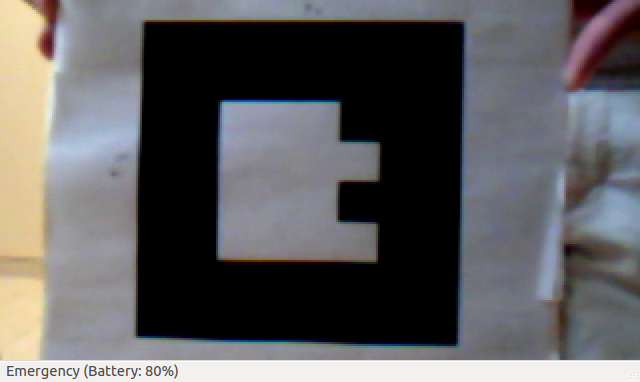
\includegraphics[width=\textwidth]{../images/min_distance.png}
			                \caption{Minimum distance for tag detection: 30cm}\label{fig:tagclose}
			        \end{subfigure}%
			        ~
			        \begin{subfigure}[b]{0.45\textwidth}
			                \centering
			                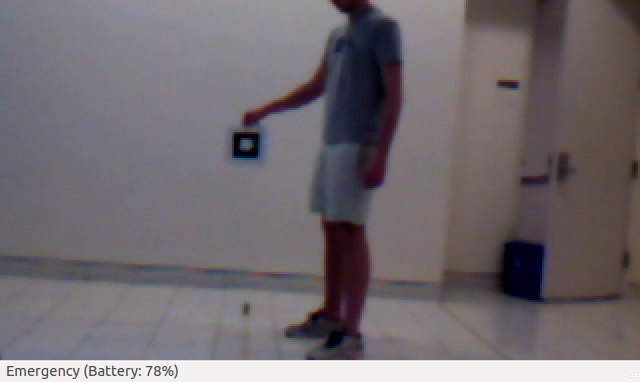
\includegraphics[width=\textwidth]{../images/max_dist2.png}
			                \caption{Maximum distance for tag detection: 4m}\label{fig:tagfar}
			        \end{subfigure}
			        \caption{Tag detection range.} \label{fig:extremes}
			\end{figure}

		\subsubsection{Tag Position Variance vs. Distance}

			In order to determine the variance of the probability density function used in the correction step, we tested the precision of the AR tag estimation algorithm at several different distances. By measuring the position of a stationary tag, we can see that the variance of measurements increases with the distance (Figure~\ref{fig:tagvar}). Interestingly, the variance along the $z$, or vertical axis, is substantially lower than that in the $x$ or $y$ axes.

			\begin{figure}[ht]
			        \centering
			        \begin{subfigure}[b]{0.32\textwidth}
			                \centering
			                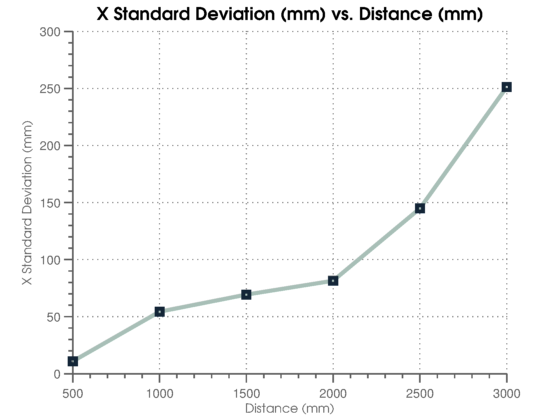
\includegraphics[width=\textwidth]{../images/artest_x.png}
			                \label{fig:tagvarx}
			        \end{subfigure}%
			        ~
			        \begin{subfigure}[b]{0.32\textwidth}
			                \centering
			                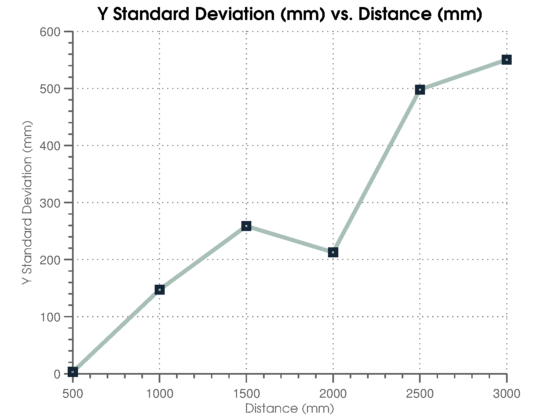
\includegraphics[width=\textwidth]{../images/artest_y.png}
			                \label{fig:tagvary}
			        \end{subfigure}
			        ~
			        \begin{subfigure}[b]{0.32\textwidth}
			                \centering
			                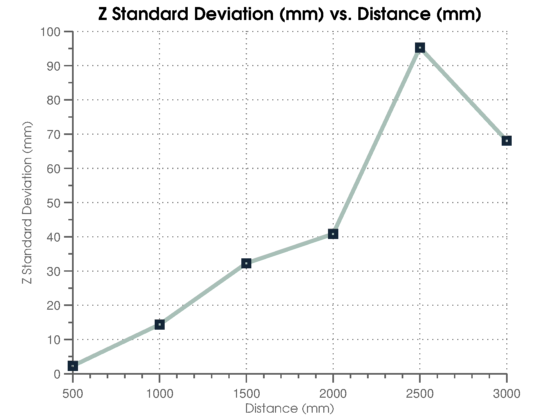
\includegraphics[width=\textwidth]{../images/artest_z.png}
			                \label{fig:tagvarz}
			        \end{subfigure}
			        \caption{Tag estimated position standard deviation.}\label{fig:tagvar}
			\end{figure}

		\subsubsection{Tag Detection Space}

			The tag detection space, which is the 3D volume above each tag in which it can be detected, is determined both by the aspect ratio and resolution of the camera and the size of the AR tag. The tag is first fully in the frame at 30cm. At an altitude of 3.5m, the area in which the tag can be detected is approximately a 2.8m by 1.8m rectangle. A result of this is that it is easier to ``hit'' a tag at a higher altitude. Therefore, it is probably best to immediately fly to a higher altitude after taking off, increasing the chance that the quadcopter will see the first tag. 

			\begin{figure}[ht]
			        \centering
			        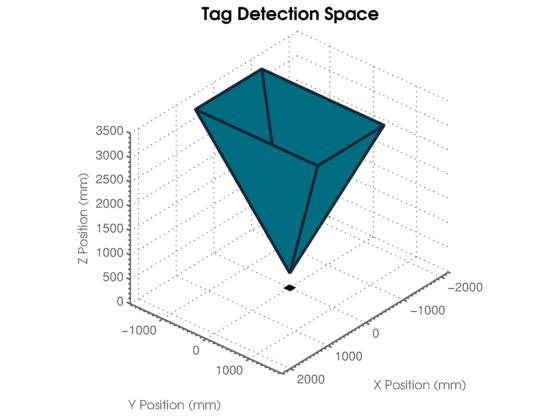
\includegraphics[width=300px]{../images/tag_detection.png}
			        \label{fig:tagdetection}
			        \caption{Tag detection space.}
			\end{figure}

		\subsubsection{Tag Detection Rate}

			We found that stationary tags were detected with a very high likelihood throughout the entire operational range. At every distance tested, the tags were correctly identified in over 98\% of frames.

		\subsubsection{Sources of Tag Error}

			We found several sources of error which could prevent the detection of AR tags. First, the movement of the quadcopter sometimes causes the camera image to be blurred as seen in Figure~\ref{fig:tagblur}. Additionally, in environments with bright overhead light, such as in direct sunlight, the quadcopter would cast a shadow over the tag, preventing it from being detected. Finally, we found that the auto-exposure of the on-board camera would often cause tags to overexpose if the background were dark, as demonstrated in Figure~\ref{fig:exposure}.

			\begin{figure}[ht]
			        \centering
			        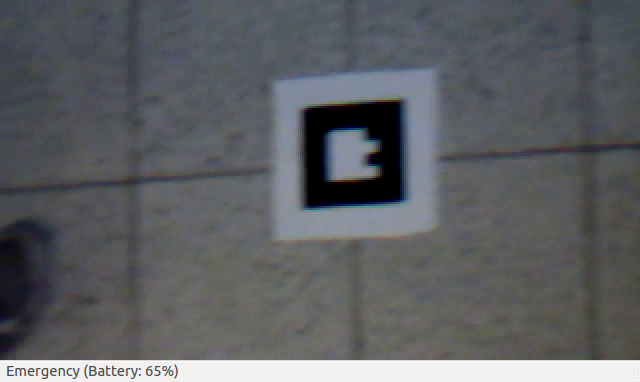
\includegraphics[width=300px]{../images/blur.png}
			        \caption{Tag motion blur.}\label{fig:tagblur}
			\end{figure}

			\begin{figure}[ht]
			        \centering
			        \begin{subfigure}[b]{0.4\textwidth}
			                \centering
			                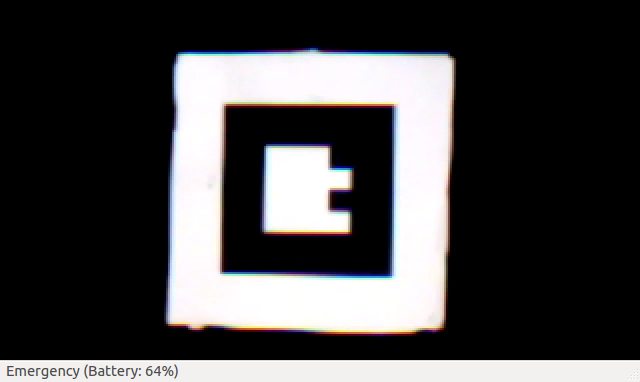
\includegraphics[width=\textwidth]{../images/exposure_good.png}
			                \label{fig:exposuregood}
			        \end{subfigure}
			        ~
			        \begin{subfigure}[b]{0.4\textwidth}
			                \centering
			                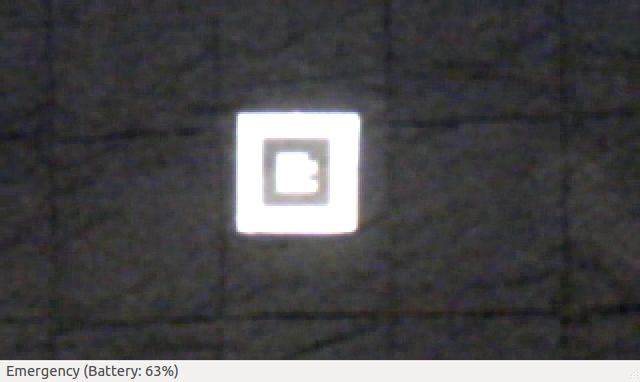
\includegraphics[width=\textwidth]{../images/exposure_bad.png}
			                \label{fig:exposurebad}
			        \end{subfigure}
			        \caption{Effect of auto-exposure on tag contrast.} \label{fig:exposure}
			\end{figure}

\section{Localization}
	
	In order to test the localization algorithm, the quadcopter was manually flown in a rectangular pattern measuring 3.5m by 2.5m. AR tags were placed at each of the corners of this pattern. Figures~\ref{fig:firsttag} through~\ref{fig:lasttag} show a comparison of localization using only visual odometry and localization using the particle filter with augmented tag correction.
	
	\begin{figure}[ht]
	        \centering
	        \begin{subfigure}[b]{0.9\textwidth}
	                \centering
	                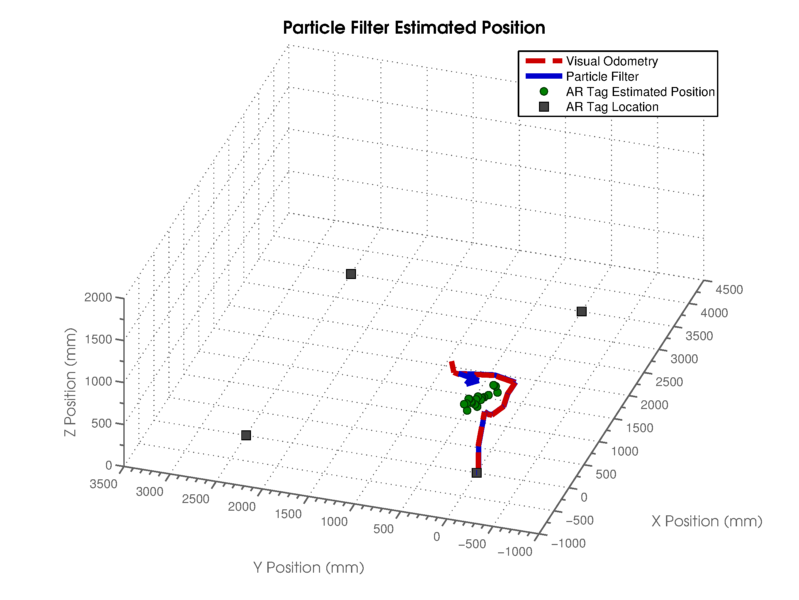
\includegraphics[width=\textwidth]{../images/3dgraph_38.png}
	                \label{fig:tag1}
	        \end{subfigure}%
	        \\
	        \begin{subfigure}[b]{0.75\textwidth}
	                \centering
	                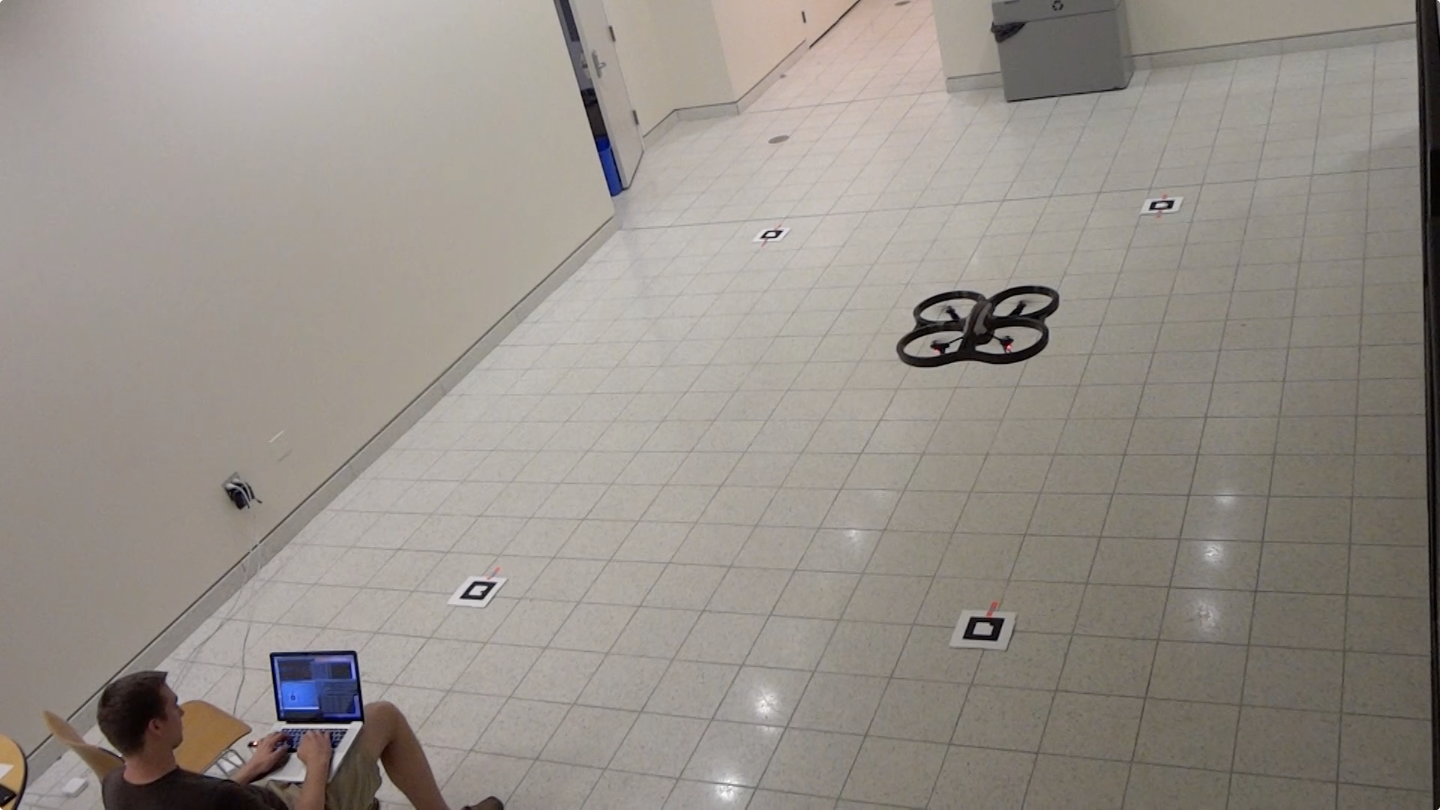
\includegraphics[width=\textwidth]{../images/frame1.png}
	                \label{fig:frame1}
	        \end{subfigure}
	        \caption{Manual flight test: first tag.} \label{fig:firsttag}
	\end{figure}

	\begin{figure}[ht]
	        \centering
	        \begin{subfigure}[b]{0.75\textwidth}
	                \centering
	                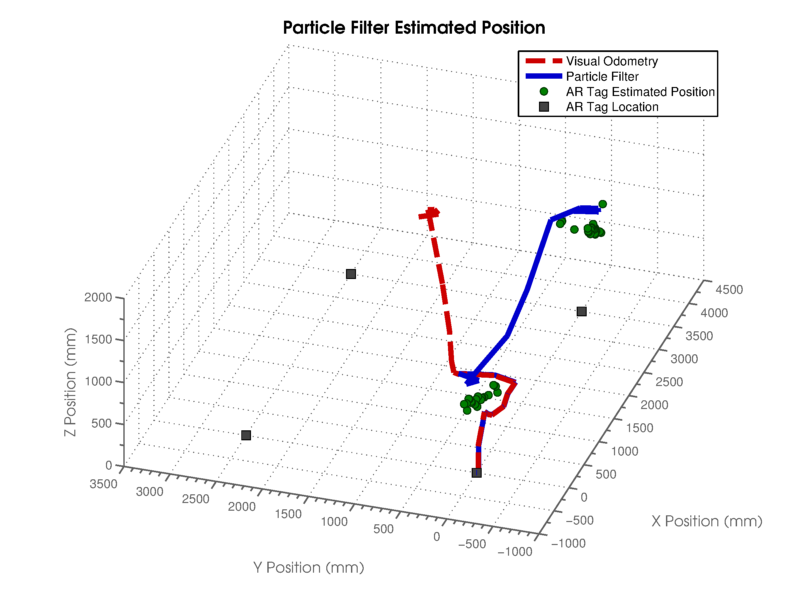
\includegraphics[width=\textwidth]{../images/3dgraph_48.png}
	                \label{fig:tag2}
	        \end{subfigure}%
	        \\
	        \begin{subfigure}[b]{0.75\textwidth}
	                \centering
	                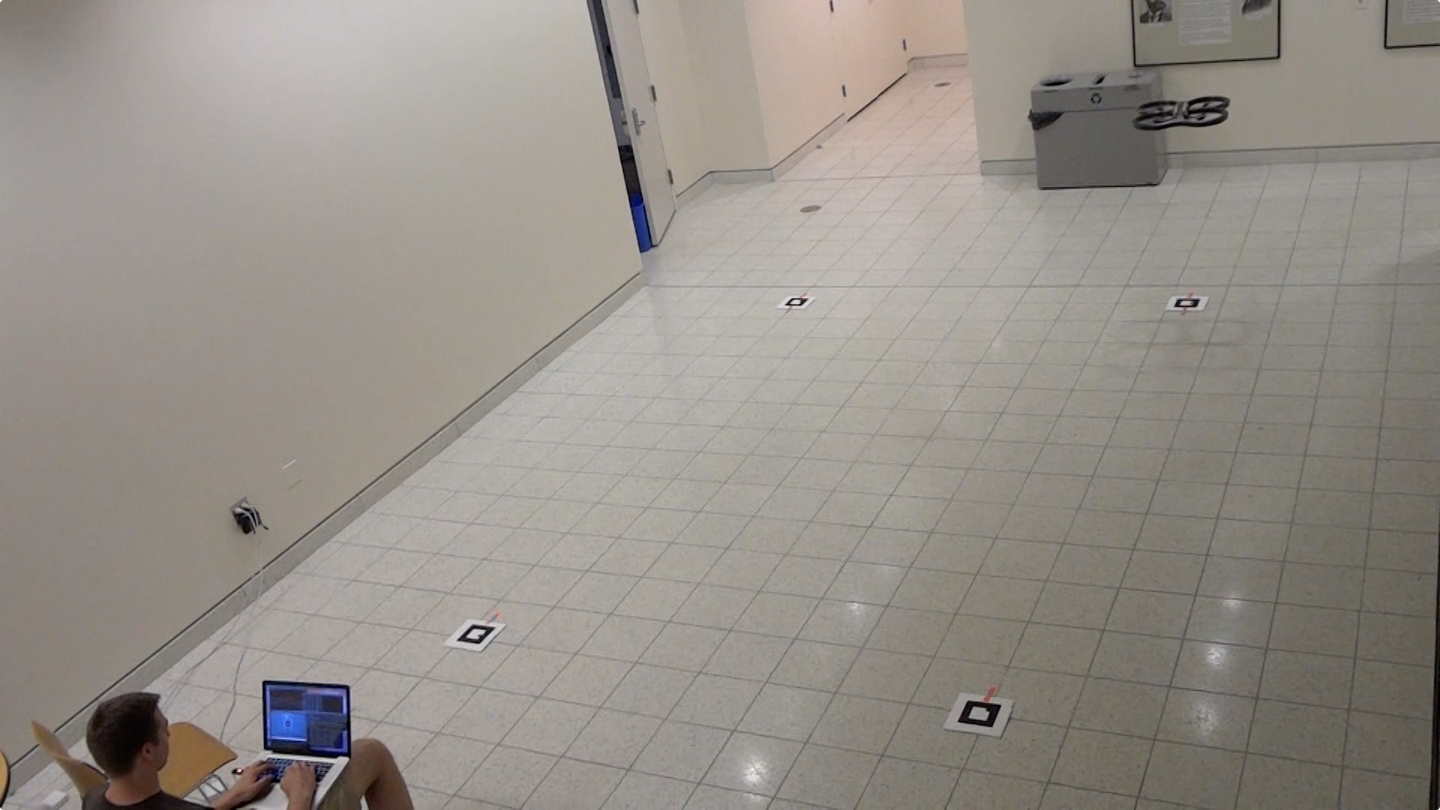
\includegraphics[width=\textwidth]{../images/frame2.png}
	                \label{fig:frame2}
	        \end{subfigure}
	        \caption{Manual flight test: second tag.}
	\end{figure}

	\begin{figure}[ht]
	        \centering
	        \begin{subfigure}[b]{0.75\textwidth}
	                \centering
	                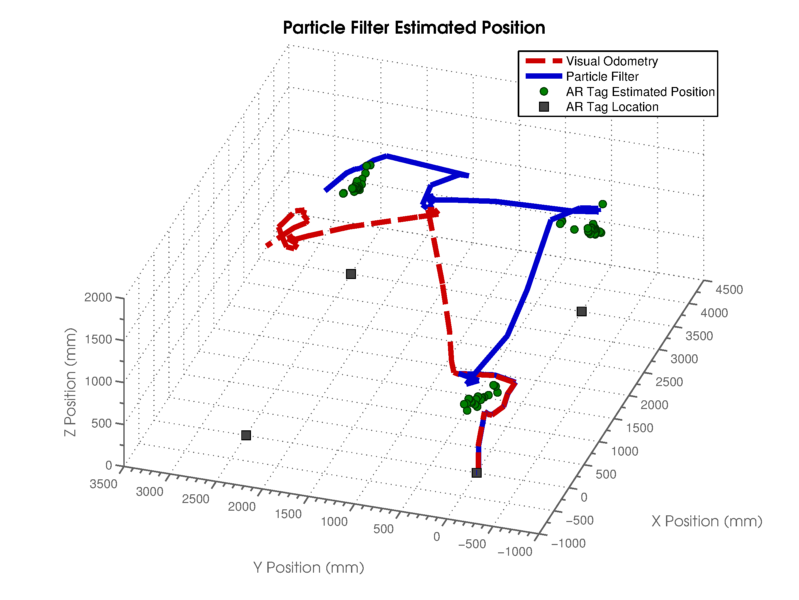
\includegraphics[width=\textwidth]{../images/3dgraph_74.png}
	                \label{fig:tag3}
	        \end{subfigure}%
	        \\
	        \begin{subfigure}[b]{0.75\textwidth}
	                \centering
	                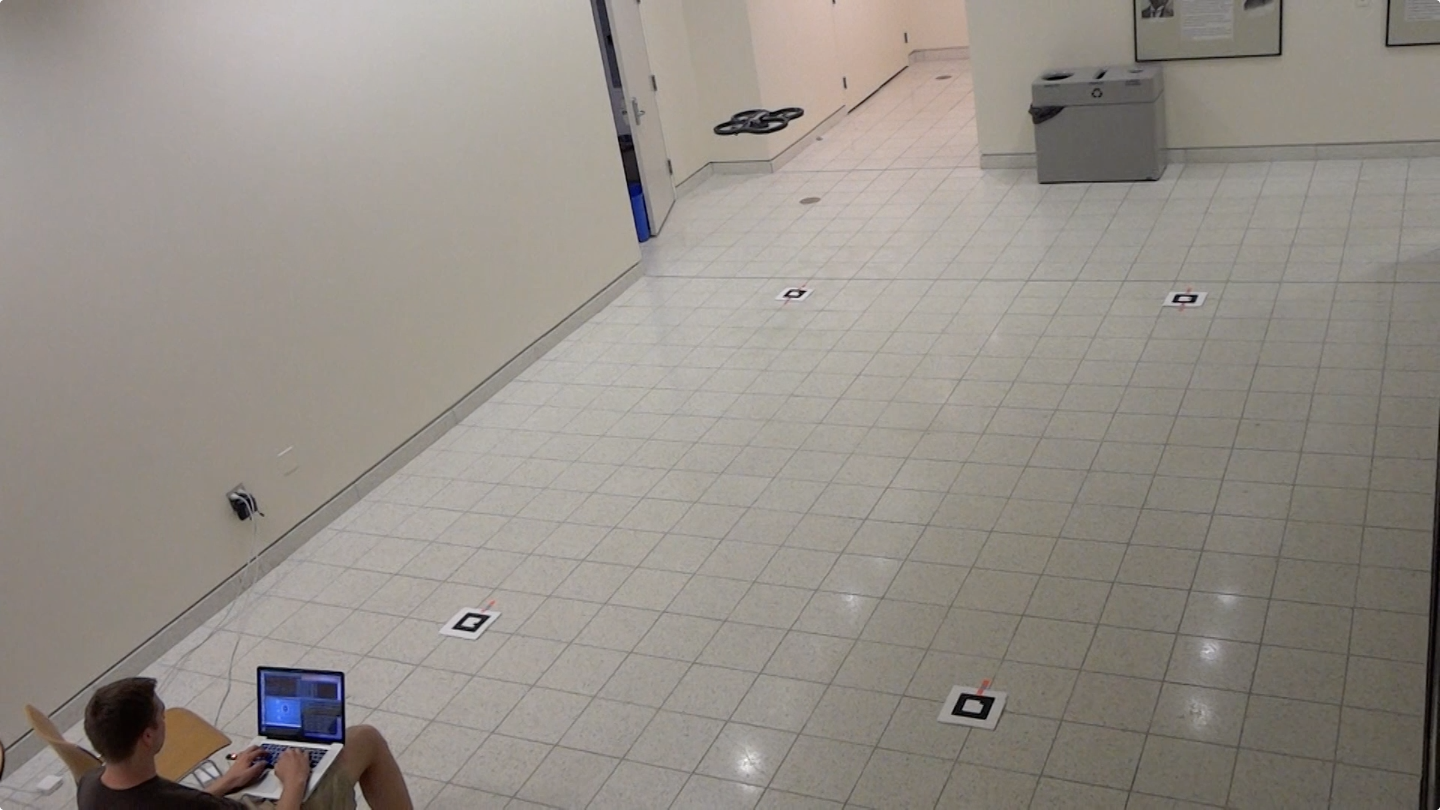
\includegraphics[width=\textwidth]{../images/frame3.png}
	                \label{fig:frame3}
	        \end{subfigure}
	        \caption{Manual flight test: third tag.}
	\end{figure}

	\begin{figure}[ht]
	        \centering
	        \begin{subfigure}[b]{0.75\textwidth}
	                \centering
	                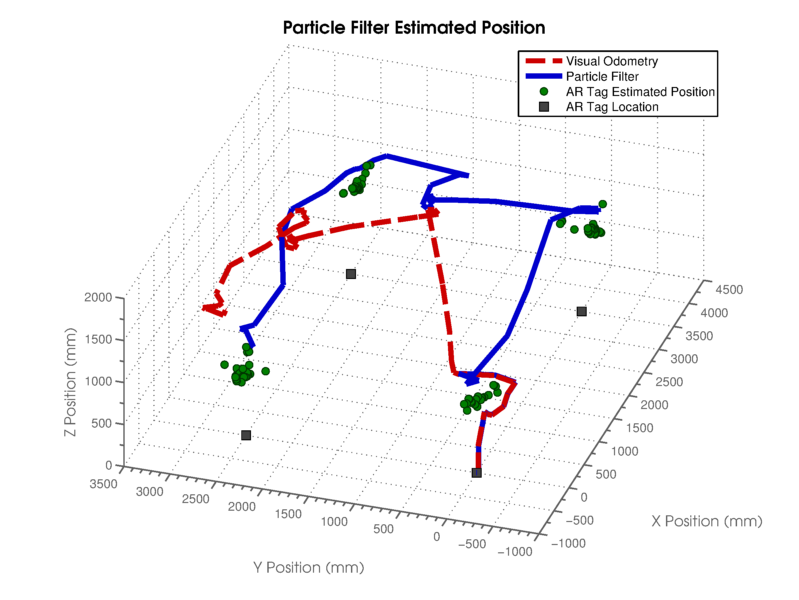
\includegraphics[width=\textwidth]{../images/3dgraph_90.png}
	                \label{fig:tag4}
	        \end{subfigure}%
	        \\
	        \begin{subfigure}[b]{0.75\textwidth}
	                \centering
	                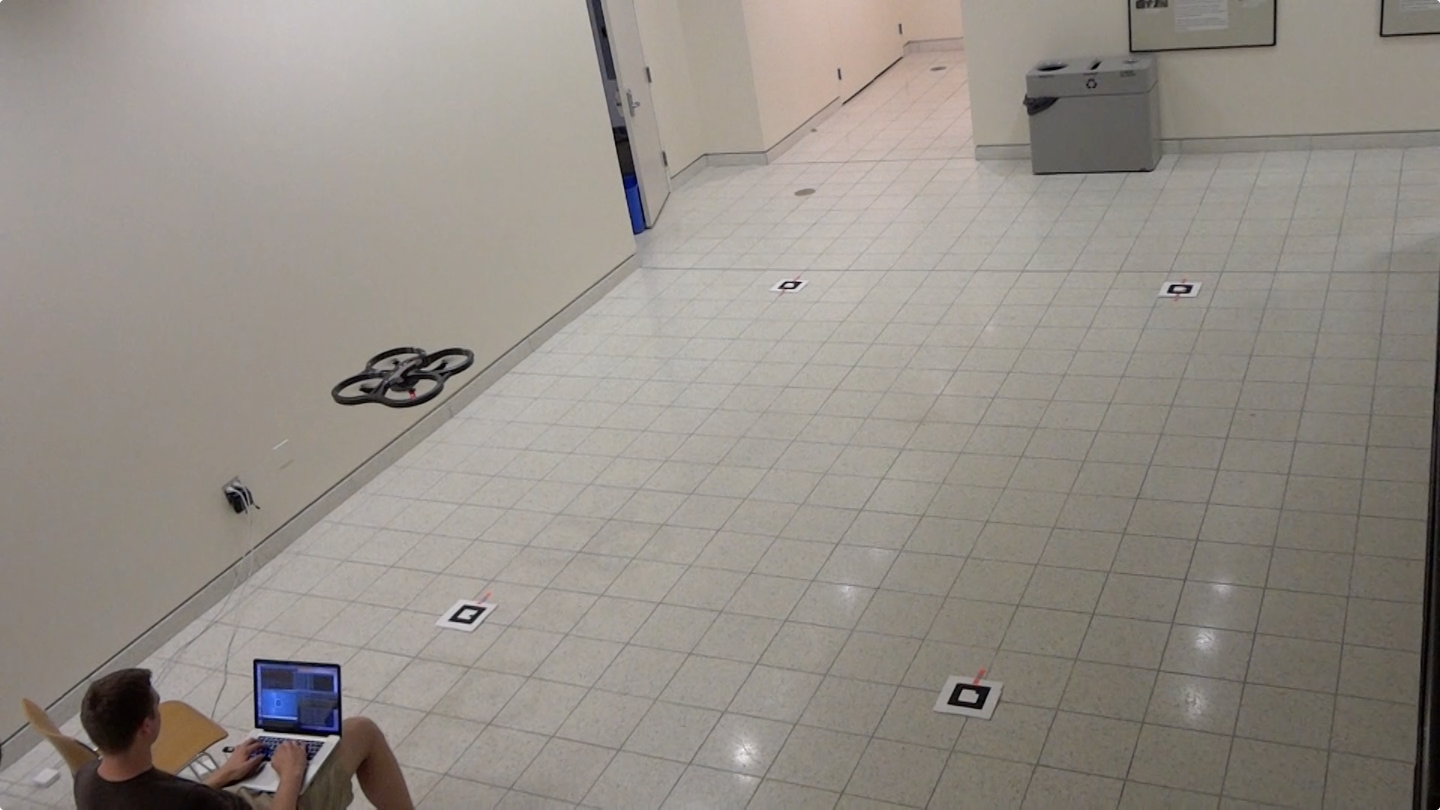
\includegraphics[width=\textwidth]{../images/frame4.png}
	                \label{fig:frame4}
	        \end{subfigure}
	        \caption{Manual flight test: fourth tag.}
	\end{figure}

	\begin{figure}[ht]
	        \centering
	        \begin{subfigure}[b]{0.75\textwidth}
	                \centering
	                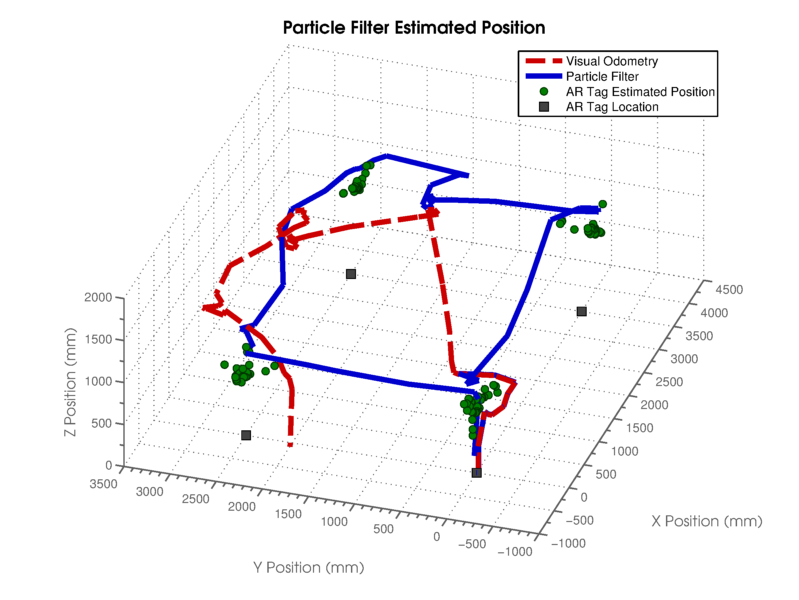
\includegraphics[width=\textwidth]{../images/3dgraph_100.png}
	                \label{fig:tag5}
	        \end{subfigure}%
	        \\
	        \begin{subfigure}[b]{0.75\textwidth}
	                \centering
	                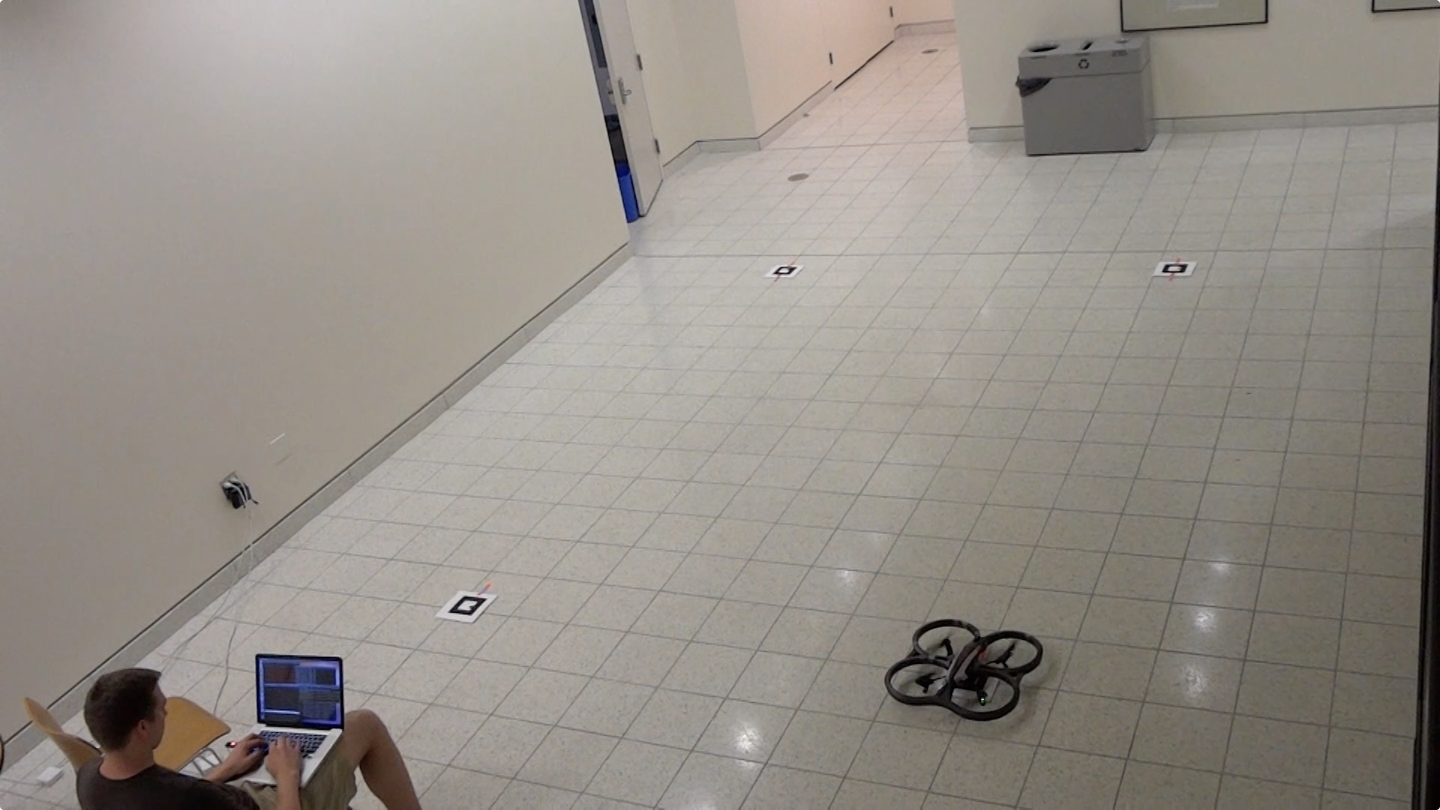
\includegraphics[width=\textwidth]{../images/frame5.png}
	                \label{fig:frame5}
	        \end{subfigure}
	        \caption{Manual flight test: final tag.}\label{fig:lasttag}
	\end{figure}

	The visual odometry measurement suffers from substantial drift, estimating that the quadcopter landed over 2m away from its actual landing location. On the other hand, the particle filter localization is able to correct for drift and accurately reflects the path of the flight.